\section{Eligibility Traces}
\begin{itemize}
	\item Eligibility traces are an alternative way of performing $n$-step TD prediction or control.
	\item $n$-step methods can be seen as \textit{forward view} algorithms that look at future rewards seen from some state and update the state value accordingly. Eligibility traces are \textit{backward view} methods that update previous state values based on how \textit{responsible} we think they were for the reward we have just obtained.
	\item They are more computationally efficient than $n$-step methods because they don't have to store the last $n$ feature vectors, but instead store one  \textit{trace} vector.
\end{itemize}

\subsection{The $\lambda$-return}
In Chapter 7 we derived the $n$-step return $G_{t:t+n}$ and used it to make updates to the state value. What if instead of using one $n$-step return, we took a weighted average of every $n$-step return? This is the $\lambda$-return and is called a \textit{compound update}, rather than a \textit{component update} in the $n$-step case. We could, for example, take the mean of the 2-step and 4-step updates, the backup diagram for which is shown in Figure \ref{fig: 12_1}.
\begin{figure}[h!]
	\centering
	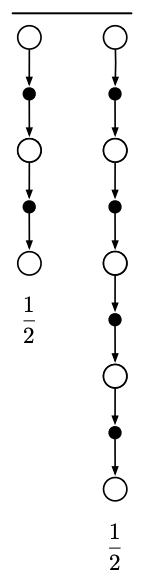
\includegraphics[width=0.1\textwidth]{/chapter12_1}
	\caption{Backup diagram for compound update for 2-step and 4-step returns}
	\label{fig: 12_1}
\end{figure}

The TD($\lambda$) algorithm generalises this approach such that each $n$-step update is weighted proportionally to $\lambda^{n-1}$ (where $\lambda \in [0, 1]$). The $\lambda$-\textit{return} in the state-based form is given by
\begin{equation} \label{eq: lambda return}
G_t^\lambda \doteq (1-\lambda) \sum_{n=1}^{\infty} \lambda^{n-1}G_{t:t+n}
\end{equation}
and the backup diagram for the algorithm is given in Figure \ref{fig: 12_2}, the decaying weighting factor is given in Figure \ref{fig: 12_3}.

\begin{figure}
	\centering
	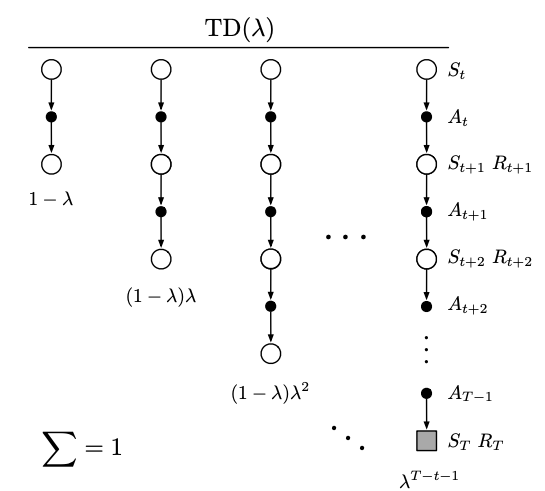
\includegraphics[width=0.6\textwidth]{/chapter12_2}
	\caption{The backup digram for TD($\lambda$). If $\lambda$ = 0, then the overall update reduces to its first component, the one-step TD update, whereas if $\lambda$ = 1, then the overall update reduces to its last component, the Monte Carlo update.}
	\label{fig: 12_2}
\end{figure}

\begin{figure}
	\centering
	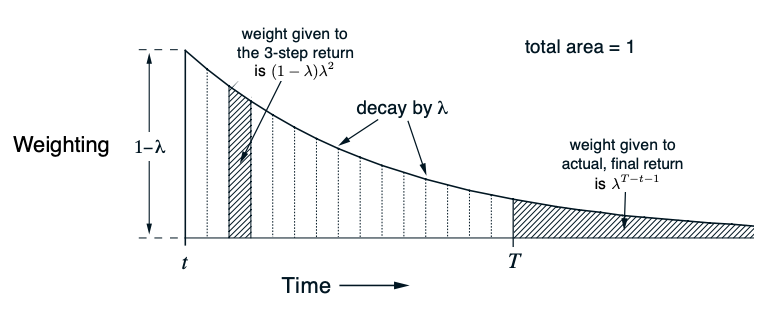
\includegraphics[width=\textwidth]{/chapter12_3}
	\caption{Weighting given in the $\lambda$-return to each of the n-step returns.}
	\label{fig: 12_3}
\end{figure}

Intuitively this algorithm makes sense. We give more responsibility for our rewards to recently selected actions and less to older selected actions, but nonetheless take into account all previously taken actions. Crucially, this algorithm is forward view, the episode is completed then we return to the first step and update based on the weighted average of all $n$-step returns received thereafter, cycling through each state.

\subsection{TD($\lambda$)}
In TD($\lambda$) the eligibility trace is first initialized to 0, and then incremented at each step by the value gradient and fades according to $\lambda$
\begin{align} \label{z}
\textbf{z}_{-1} &\doteq \textbf{0} \\
\textbf{z}_t &\doteq \gamma \lambda \textbf{z}_{t-1} + \nabla \hat{v}(S_t, \textbf{w}_t)
\end{align}

here the value gradient is effectively a proxy for the state visited i.e. bump up the eligibility at these weights because a state corresponding to these weights has been visited recently. We know the TD error for state-value prediction is
\begin{equation}
\delta_t \doteq R_{t+1} + \gamma \hat{v}(S_{t+1}, \textbf{w}_t) - \hat{v}(S_t, \textbf{w}_t)
\end{equation}

and the weight vector in TD($\lambda$) is updated in proportion to the TD error and the eligibility trace
\begin{equation}
\textbf{w}_{t+1} \doteq \textbf{w}_t + \alpha \delta_t \textbf{z}_t
\end{equation}

The algorithm for semi-gradient TD($\lambda$) is given in Figure \ref{fig: 12_4}
\begin{figure}
	\centering
	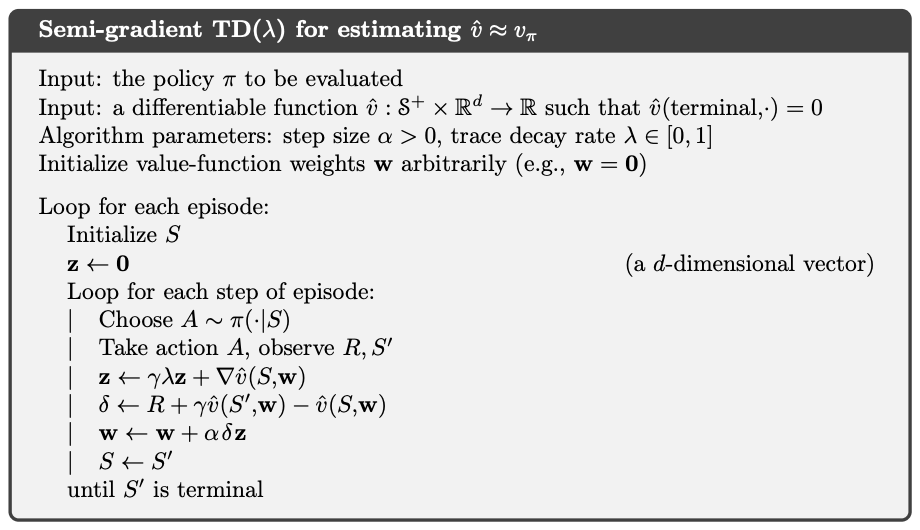
\includegraphics[width=0.8\textwidth]{/chapter12_4}
	\caption{Pseudocode for semi-gradient TD($\lambda$)}
	\label{fig: 12_4}
\end{figure}

To understand TD($\lambda$) better lets consider the extreme cases of $\lambda = 0$ and $\lambda = 1$. In the former, the algorithm becomes one step returns as per TD(0) discussed in chapter 6. In the later we get Monte Carlo returns where every single previous state is updated with the return, but discounted by $\gamma$. (Note: this gives insight as to why $\gamma$ is still retained in equation \ref{z}). The advantage of this kind of Monte Carlo return, as compared with the normal MC return discussed in chapter 5, is that it can be performed \textit{online} rather than waiting for the end of the episode before backpropogating the returns.

\subsection{$n$-step Truncated $\lambda$-return Methods}
The off-line $\lambda$-return algorithm, which uses the $\lambda$-return (Equation \ref{eq: lambda return}), is an important ideal but of little use in the episodic case (because we have to wait until the end of the episode before we make any updates), nor the continuing case (because it cannot be calculated for arbitrarily large $n$). Instead we can use the truncated $\lambda$-return which halts the return calculation at some horizon $h$:
\begin{equation} \label{eq: horizon}
G_{t:h}^\lambda \doteq (1 - \lambda) \sum_{n=1}^{h - t - 1} \lambda^{n-1} G_{t:t+n} + \lambda^{h-t-1}G_{t:h}, \; \; \; 0 \leq t < h \leq T
\end{equation}

\subsection{Redoing Updates: Online $\lambda$-return Algorithm}
The problem with the algorithm described in the last section is the choice of truncation parameter $n$. If it is too small, then we do not get the benefit of the offline $\lambda$-return algorithm that uses all $n$ step updates from an episode, and if it is too large then we cannot learn quickly online. We can, in principle, get the best of both using the \textit{online $\lambda$-return algorithm}, but we pay for this with computational complexity.

For every step we take in an episode, we recalculate the $\lambda$-return for the whole episode, where our current step acts as horizon $h$ in equation \ref{eq: horizon}. We are then making increasingly accurate updates to states as we move through the episode, but the number of calculations required at each step scales with $n$. The updates are given in Figure \ref{fig: 12_5}.
\begin{figure}
	\centering
	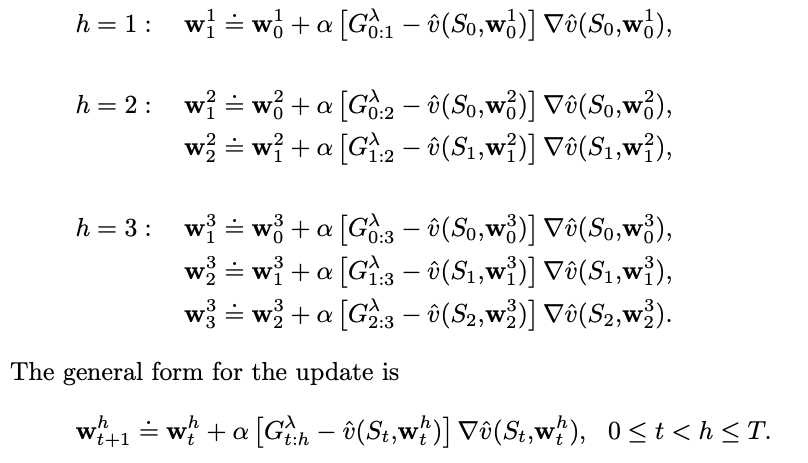
\includegraphics[width=0.6\textwidth]{/chapter12_5}
	\caption{Online $\lambda$-return updates for the first three steps of an episode}
	\label{fig: 12_5}
\end{figure}

In general, online $\lambda$-return performs better than off $\lambda$-return because it has had more, informative updates the weight vector used for bootstrapping throughout the episode. Note: this is a forward view algorithm, we keep updating state values by looking at a stream of future rewards as they are updated 

\subsection{True Online TD($\lambda$)}
\begin{itemize}
\item We can produce a backward view version of the online $\lambda$-return algorithm presented in the last section that uses eligibility traces, called True Online TD($\lambda$).
\item Because of a trick with the weight matrix, where we only need to keep the last weight vector from all the updates at the last time step, the computational complexity of True Online TD($\lambda$) matches TD($\lambda$).
\item The pseudocode for True Online TD($\lambda$) is given in Figure \ref{fig: 12_6}.
\end{itemize}
\begin{figure}
	\centering
	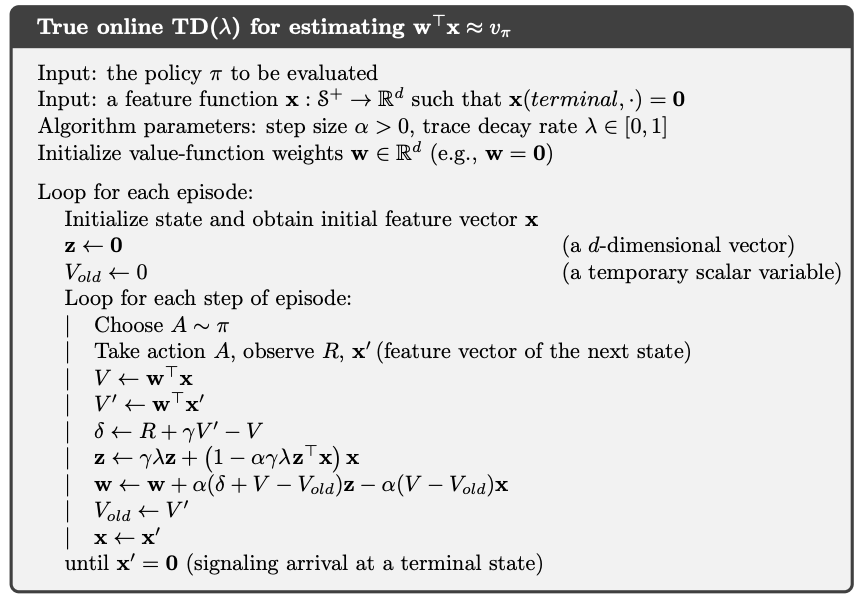
\includegraphics[width=0.8\textwidth]{/chapter12_6}
	\caption{True Online TD($\lambda$)for estimating $\textbf{w}^T\textbf{x} \approx v_\pi$}
	\label{fig: 12_6}
\end{figure}

\subsection{SARSA($\lambda$)}
We can extend the ideas discussed in this chapter (i.e. eligibility traces) to the action-value, forward-view case readily, producing the SARSA($\lambda$) algorithm. The full list of equations required for SARSA($\lambda$) are detailed below. First we need the action-value form of the $n$-step return
\begin{equation}
G_{t:t+n} \doteq R_{t+1} + \cdots + \gamma^{n-1} R_{t+n} + \gamma^n \hat{q}(S_{t+n}, A_{t+n}, \textbf{w}_{t+n-1}), \; \; \; t+n < T,
\end{equation}
with $G_{t:t+n} \doteq G_t$ if $t+n \geq T$. The action-value form of the offline $\lambda$-return algorithm simply use $\hat{q}$ rather than $\hat{v}$:

\begin{equation}
\textbf{w}_{t+n} \doteq \textbf{w}_{t+n-1} + \alpha \left[G_{t}^\lambda - \hat{q} (S_t, A_t, \textbf{w}_{t+n-1})\right] \nabla \hat{q}(S_t, A_t, \textbf{w}_{t+n-1}), \; \; \; t=0, \ldots, T-1
\end{equation}
where $G_{t}^\lambda \doteq G_{t: \infty}^\lambda$.  The algorithm has the same update rule as given earlier for TD($\lambda$)
\begin{equation}
\textbf{w}_{t+1} \doteq \textbf{w}_t + \alpha \delta_t \textbf{z}_t
\end{equation}
except it uses the action-value form of the TD error:
\begin{equation}
\delta_t \doteq R_{t+1} + \gamma \hat{q}(S_{t+1}, A_{t+1}, \textbf{w}_t) - \hat{q}(S_t, A_{t}, \textbf{w}_t),
\end{equation}
and the action-value form of the eligibility trace:
\begin{align} \label{z}
\textbf{z}_{-1} &\doteq \textbf{0} \\
\textbf{z}_t &\doteq \gamma \lambda \textbf{z}_{t-1} + \nabla \hat{q}(S_t, A_{t}, \textbf{w}_t), \; \; \; 0 \leq t \leq T.
\end{align}

Complete pseudocode for the algorithm is given in Figure \ref{fig: 12_7}.

\begin{figure}
	\centering
	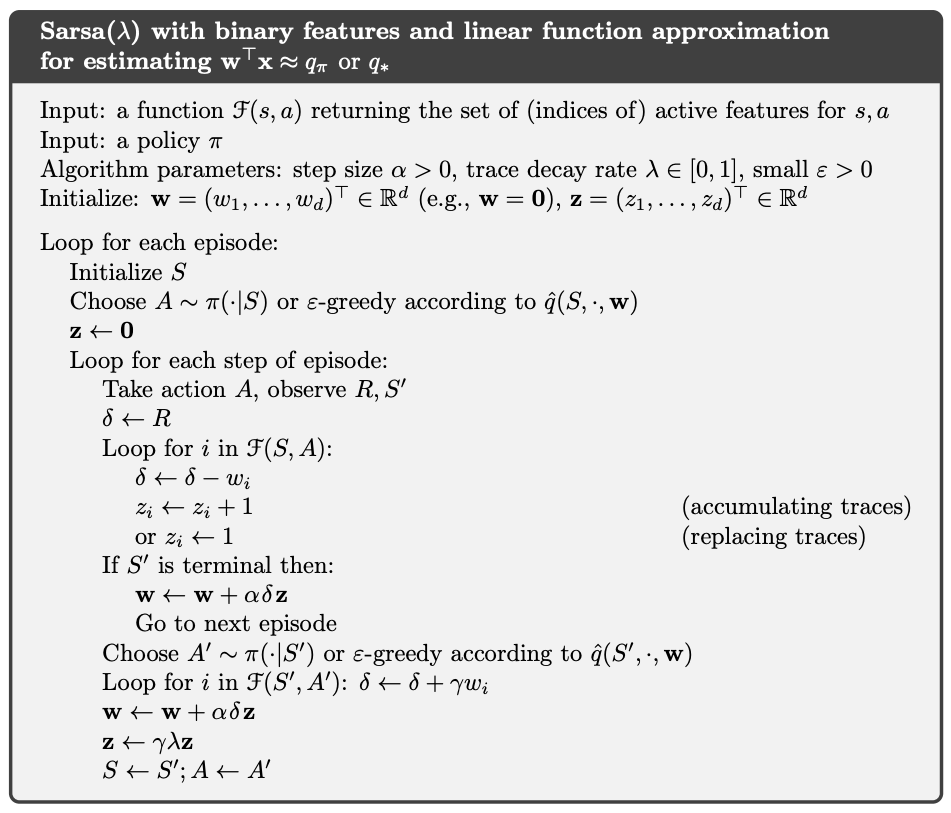
\includegraphics[width=0.8\textwidth]{/chapter12_7}
	\caption{SARSA($\lambda$) with binary features and linear function approximation for estimating $w^T \approx q_\pi or q_*$}
	\label{fig: 12_7}
\end{figure}

A compelling visual description of the different SARSA algorithms reviewed thus far is given in Figure \ref{fig: 12_8}. The SARSA($\lambda$) updates make the most intuitive sense. It is the actions closest to the final reward where we can be most confident in their value, actions prior to the goal may have had a direct effect in producing the reward, but the distance between action and target means there is uncertainty in how much that action affected the final outcome. Consequently, updating the values of these actions more conservatively appears rational. SARSA($\lambda$) proves the most efficient and learning optimal policies in these settings for this reason.

To explain clearly the intuition behind this algorithm we refer back to Figure \ref{fig: 12_3}. If we imagine ourselves in the first state and observe the weight we give to all forthcoming updates, we see that we give the bulk of the weight to the initial rewards we receive (0 in the gridworld) and the least weight to the final return at time $T$. Equally, if we are in the final state prior to termination, we give most weight to the next-step rewards (1 in the gridworld). This creates the fading reward traces shown in Figure \ref{fig: 12_7}.

\begin{figure}
	\centering
	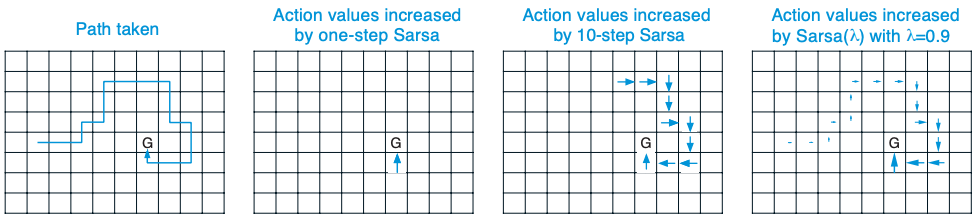
\includegraphics[width=0.8\textwidth]{/chapter12_8}
	\caption{4 SARSA algorithms tackling the gridworld task}
	\label{fig: 12_8}
\end{figure}

\subsection{Variable $\lambda$ and $\gamma$}
We can amend $\lambda$, the eligibility trace parameter, and $\gamma$, the discounting parameter, to vary with state rather than be constants throughout an episode. That is, $\lambda$ and $\gamma$ are now state-dependent and denoted $\lambda_t$ and $\gamma_t$. This creates a further layer of generalisation not yet seen. The return is now defined more generally as
\begin{align}
	G_t &\doteq R_{t+1} + \gamma_{t+1}G_{t+1} \\
	&= R_{t+1} + \gamma_{t+1}R_{t+2} + \gamma_{t+1}\gamma_{t+2}R_{t+3} + \cdots \\
	&= \sum_{k=t}^{\infty} \left(\prod_{i=t+1}^{k} \gamma_i\right) R_{k+1} \\
\end{align}

\subsection{Off-policy Traces with Control Variates}
To generalise to the off-policy case we need to bring back ideas from importance sampling. This section, and associated derivations, are long, but eventually we arrive at a new eligibility trace
\begin{equation}
\textbf{z}_t \doteq \gamma_t \lambda_t \rho_t \textbf{z}_{t-1} + \nabla \hat{q}(S_t, A_t, \textbf{w}_t), 
\end{equation}
where $\rho_t = \frac{\pi(A_t | S_t)}{b(A_t | S_t)}$ is the single-step importance sampling ratio.

\subsection{Watkins's Q($\lambda$) to Tree-Backup($\lambda$)}
Q-learning and Tree-backups can be extended to the eligibility trace setting too, and are called Watkins's Q($\lambda$) and Tree-backup($\lambda$) respectively. Their backup diagrams are shown in Figures \ref{fig: 12_9} and \ref{fig: 12_10}. In Q($\lambda$) we continue to include weighted $n$-step rewards whilst greedy actions are selected, but when a non-greedy action is selected on-policy the cumulative reward terminates with an expectation at that state.

\begin{figure}
	\centering
	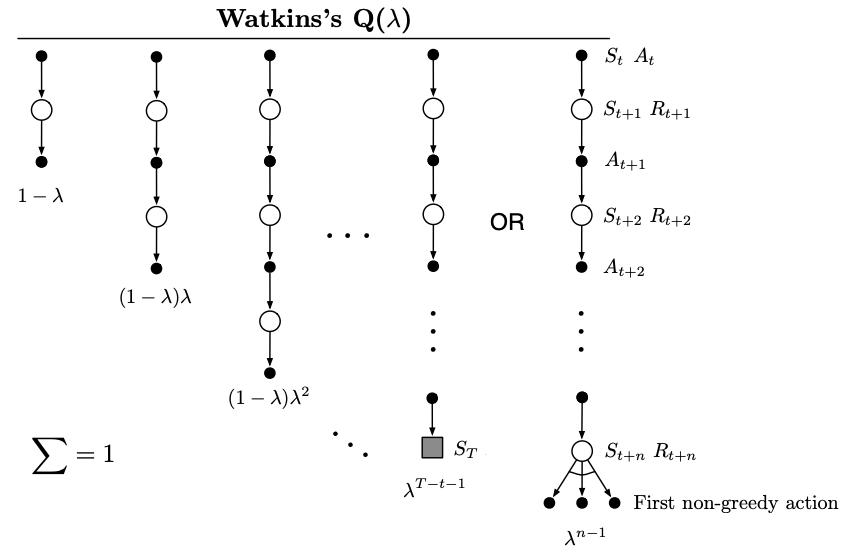
\includegraphics[width=0.8\textwidth]{/chapter12_9}
	\caption{The backup diagram for Watkins’s Q($\lambda$). The series of component updates ends either with the end of the episode or with the first non-greedy action, whichever comes first.}
	\label{fig: 12_9}
\end{figure}

\begin{figure}
	\centering
	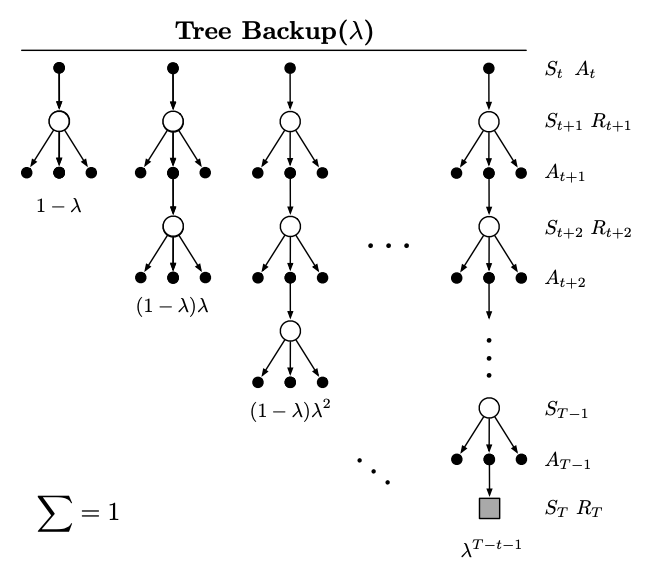
\includegraphics[width=0.7\textwidth]{/chapter12_10}
	\caption{The backup diagram for the $\lambda$ version of the Tree Backup algorithm.}
	\label{fig: 12_10}
\end{figure}

\subsection{Implementation Issues}
In the tabular setting, it would appear that every state-value instance would need to be updated at every timestep. This is a problem for implementation on traditional serial computers. Fortunately, for typical values of $\lambda$ and $\gamma$, almost all state have eligibility traces near zero. In practice, therefore, we only need to update the states for which the update is some margin bigger than zero, decreasing the complexity of the system. Function approximation, like ANNs, reduce the complexity of eligibility-based algorithms too.

\subsection{Key Takeaways}
\begin{itemize}
\item Eligibility traces allow us to walk the continuum between one-step methods and Monte Carlo in a similar way to the $n$-step methods discussed in chapter 7. They are, however, more general, and learn value functions more quickly.
\item Monte Carlo methods are good in non-Markov environments, because their rewards are unbiased by bootstrapping. Eligibility traces have the same property. They are most useful for environments that have long-delayed rewards and are non-Markov.
\item Eligibility traces use significantly more computation than $n$-step methods, but in return they offer significantly faster learning, particularly when rewards are delayed by many steps. Thus they can be particularly effective in \textbf{low data settings}, and not effective when data can be acquired cheaply via a simulator. When data is cheap, the challenge is processing that data as quickly as possible, and typically, that means using one-step methods like Q-learning.
\item $\lambda$-return is forward view and TD($\lambda$) is backward view.
\end{itemize}


